\chapter{Probleme}
Die meisten Probleme entstanden bei der Annahme es gäbe Konsistenz in der Formatierung der Dokumente (siehe \autoref{ch:solution}, \autopageref{ch:solution}). 
\section{Dokumenttyp}
Erste Probleme tauchten noch vor der eigentlichen Extraktion auf, nämlich beim Einlesen der Plenarprotokolle in XML Form auf.
\begin{figure}[h]
	\begin{minipage}{.48\linewidth}
		\caption*{Mit Angabe des Dokumententyps}
		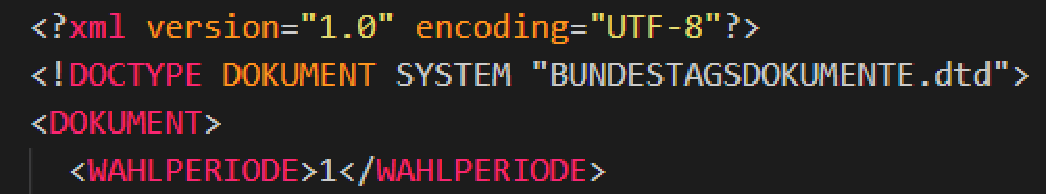
\includegraphics[width=\linewidth]{img/withdoctype.pdf}		
	\end{minipage}\hfill
	\begin{minipage}{.48\linewidth}
		\caption*{Ohne Angabe des Dokumententyps}
		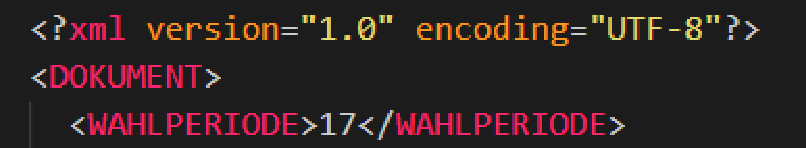
\includegraphics[width=\linewidth]{img/withoutdoctype.pdf}
	\end{minipage}
	\caption{Unterschiede in der Angabe des Dokumententyps}
	\label{img:doctype}
\end{figure}\\
In der 1. - 14. Wahllegislaturperiode wurden den XML-Dateien ein Dokumententyp angegeben, ab der 15. Wahllegislaturperiode war die nicht mehr der Fall. Beipielhaft wird dies in \autoref{img:doctype} durch ein Ausschnitt eines Protokolls der 1. und eines der 17. Wahllegislaturperiode verdeutlicht.

\section{Formatierung}
\begin{figure}[h]
	\begin{minipage}{.49\linewidth}
		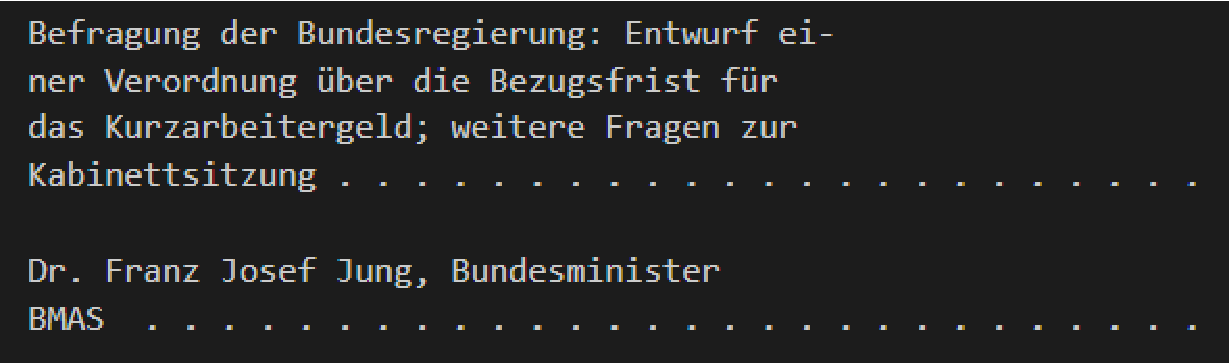
\includegraphics[width=\linewidth]{img/toc17.pdf}
	\end{minipage}\hfill
	\begin{minipage}{.49\linewidth}
		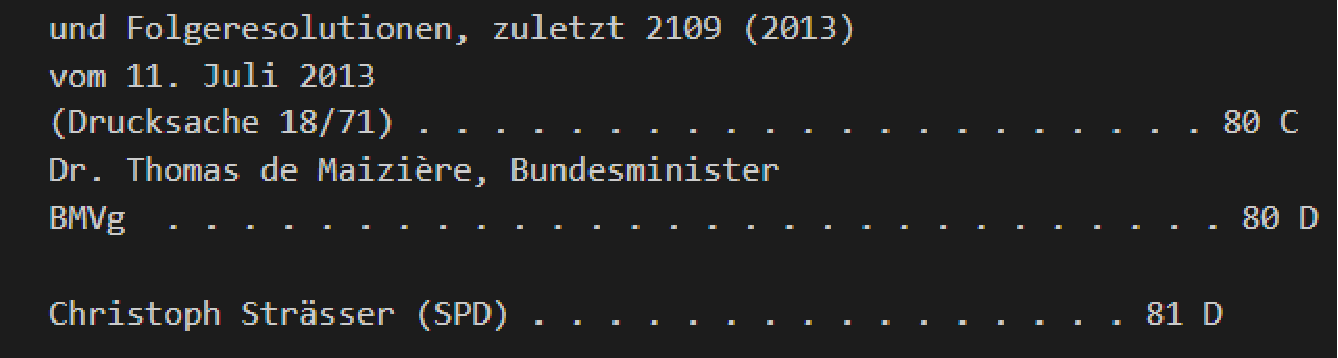
\includegraphics[width=\linewidth]{img/toc18.pdf}
	\end{minipage}
	\caption{Unterschiede in der Darstellung des Inhaltsverzeichnisses}
	\label{img:diffenzeToc}
\end{figure}

\noindent
Durch weitere Testdurchläufe wurde ein deutlicher Unterschied in den Inhaltsverzeichniseinträgen gefunden (siehe \autoref{img:diffenzeToc}), womit die Benutzung des trennenden regulären Ausdruckes nicht für alle Dokumente möglich war.  Des Weiteren ist die scheinbare Gemeinsamkeit der Punkte nicht in alle Dokumenten gegeben.\\

\newpage
\section{Benamung der Zugehörigkeit}
Auch bei Benamung von Zugehörigkeiten gab es viele Unterschiede in der Schreibweise. Bestes Beispiel ist hierfür die Partei \gequote{BÜNDNIS 90/DIE GRÜNEN}. Allein für die unterschiedlichen Schreibweisen dieser Partei:
\begin{multicols}{2}
	\begin{itemize}
		\item BÜNDNIS 90/DIE GRÜNEN
		\item BÜNDNIS 90/\\
		DIE GRÜNEN
		\columnbreak
		\item BÜNDNIS 90/\\
		
		DIE GRÜNEN
		\item BÜNDNIS 90/DIE GRÜ-\\
		NEN	
	\end{itemize}
\end{multicols}
mussten drei reguläre Ausdrücke abgeändert werden damit sie funktionieren.

\section{Personensuche im Inhaltsverzeichnis}
Der entscheidende Punkt bei der Extraktion war die Suche im Inhaltsverzeichnis nach Personen. Innerhalb der Suche selbst gab es aber Unterschiede die separat abgearbeitet werden mussten.\\
Die Suche wurde mit der Methode \lstinline|createMap()| in der \lstinline|SpeechSearch|-Klasse implementiert. Der wörtlich Ablauf der Methode sieht grob wie folgt aus:
\begin{itemize}[leftmargin=3.5em]
	\item[\textbf{Wenn}] es einen Titel \gequote{Geschäftsordnung} gibt,
	\begin{itemize}
		\item[\textbf{dann}] ist im selben Eintrag auch der erste Name enthalten und muss gespeichert werden
		\item[] danach ist jeder Eintrag ein Name,
		\item[] bis zum Eintrag der einen Titel enthält.
		\item[] nächster Schleifendurchlauf ab dem Titel.
	\end{itemize}
	\item[\textbf{sonst}] ,
	\begin{itemize}
		\item[\textbf{wenn}] nach einem Titel ein Name folgt
		\begin{itemize}
			\item[\textbf{dann}] ist jeder nachfolgende Eintrag ein Name und muss gespeichert werden,
			\item[] bis ein Eintrag einen Titel enthält
			\item[] nächster Schleifendurchlauf ab dem Titel.
		\end{itemize}
	\end{itemize}
\end{itemize}
Wurden zu jedem Titel die Redner gefunden, werden diese Einträge in einer \lstinline|Map| gespeichert.

